%!TEX root = ../report.tex

\todo{Purpose of the chapter
 Structure of the chapter
 Central themes of the chapter}

\section{Development environment} {
\label{sec:development_environment}

	The tools and libraries used for the development environment of this project have been outlined in Table~\ref{tab:development_environment}.

	\begin{table}[H]
\caption[Development environment]{The list of project dependencies for the development environment.}
\label{tab:development_environment}
\begin{tabularx}{\textwidth}{@{}XX@{}}
	\toprule
	\textbf{Dependency} & \textbf{Description} \\
	\midrule
	Git & Version control \\
	BitBucket & Source code host \\
	SourceTree & Git client \\
	IntelliJ IDEA & Integrated development environment \\
	Node.js & Runtime environment \\
	Three.js & WebGL abstraction library \\
	RequireJS & Dependency injection library \\
	\bottomrule
\end{tabularx}
\end{table}

}

\section{Software configuration management} {
\label{sec:software_configuration_management}

	\emph{Git} is a distributed revision control system that has been used throughout the course of this project. Its primary function is to manage changes in the source code, but also to maintain any associated documentation for this project. The key advantages of using this system are as follows:

	\begin{itemize}
		\item Emphasis on speed and scale.
			\begin{itemize}
				\item Can support thousands of contributors.
			\end{itemize}
		\item Provides great flexibility towards workflows.
		\item Low storage requirements.
		\item It is decentralised.
			\begin{itemize}
				\item Promotes offline work because everybody has their own repository.
			\end{itemize}
	\end{itemize}

	It is important to note that a decentralised system is superior to other revision control systems, in that changes can be saved locally and then later be added to the remote repository. On the other hand, a centralised system such as Subversion, requires users to physically copy their changes in code when the network location is out of reach.

	While this project is being implemented by a single developer, it is essential to consider future work and the possibility of having more contributors. By using Git as a means of revision control, this should not become an issue due to its sheer scalability.

}

\section{CSS} {
\label{sec:css}

	Less is a CSS pre-processor that extends the CSS language by allowing variables, mixins, functions and other techniques to generate CSS that is more maintainable, themable and extendable~\footnote{\bibentry{sellier2009less}}. Less was used in this project over Sass due to its simplicity. Sass is more powerful than Less, but requires the installation of Ruby to compile \texttt{scss} files. Less is more intuitive than Sass and incorporates all the necessary features that would be used in this project. Consequently, this makes Less the more feasible and optimal solution for creating CSS.

}

\section{Libraries} {
\label{sec:libraries}
	
	\subsection{Node.js} {
	\label{sec:nodejs}
	
		Node.js is an open-source, cross-platform runtime environment for network applications. It uses an event-driven architecture and non-blocking I/O model that makes it lightweight and efficient~\footnote{\bibentry{nodejs2009node}}. This platform is ideal for web projects due to its simplicity and quick deployment time, as an application can be created, built and run in a matter of minutes.

	}

	\subsection{Three.js} {
	\label{sec:threejs}

		Three.js~\footnote{\bibentry{cabello2010three}} is a JavaScript library that abstracts WebGL and was used for developing the visualisations. It is superior to other WebGL frameworks because of its strong communnity, well-structured codebase, extensive set of features and examples that can be integrated into any project. Libraries such as SceneJS are not designed for rendering complex scenes, while GLGE and other available libraries are less feature complete. Therefore, this makes Three.js a great candidate for developing this project.

	}

	\subsection{RequireJS} {
	\label{sec:requirejs}
		
		RequireJS is a JavaScript file and module loader~\footnote{\bibentry{chung2011requirejs}} that can be used as a dependency injection library. This library promotes the use of modules, so a JavaScript application can resemble a typical class structure in other languages. It also has an optimiser that can generate a single script for the entire application, which can be used in production mode.

	}

	\subsection{Handlebars} {
	\label{sec:handlebars}

		Handlebars is a JavaScript web templating system that was used for the information displays in this project. It is built on top of Mustache, which is often considered a base for JavaScript templating\footnote{\bibentry{franklin2013template}}. This templating system was preferred to others because it is widely used, has a large community and helper methods can be registered and accessed within a template. Furthermore, this same library was also in the group project, increasing consistency and integration between the systems.

		The information displays could have also been generated by dynamically creating HTML in the client side. However, this method is less elegant and harder to configure. The use of HTML templates facilitates a clean, structured syntax which has been obtained by using Handlebars.

	}

	\subsection{Material Design framework} {
	\label{sec:material_design_framework}

		There are several CSS3 Material Design frameworks available such as Material Design for Bootstrap, Material Design Lite and Materialize. Each framework has been examined below.

		\emph{Material Design for Bootstrap} is a theme for Bootstrap 3, which lets you use Google Material Design on top of Bootstrap~\footnote{\bibentry{vrasta2014material}}. It is currently used in the group project, but it is a bloated framework and requires the following:

		\begin{verbatim}
			jquery.min.js 		29.3KB
			bootstrap.min.css 	19.2KB 
			material.min.css 	23.9KB
			material.min.js 	1.6KB
		\end{verbatim}

		This totals \texttt{74KB} gzipped, which is a reasonably large strain on the network for loading a single library on a system that targets good performance.
		
		\emph{Material Design Lite} is a lightweight Material Design framework, that doesn't rely on any JavaScript frameworks~\footnote{\bibentry{google2014materialdesignlite}}. It provides a good variety of components, including a sliding drawer which other Material Design frameworks do not support. However, this framework has a bloated syntax and the drawer could not be configured precisely as intended. It is also extremely difficult to change colour schemes when installing this framework on your own server.

		\emph{Materialize} is a modern, responsive front-end framework based on Material Design~\footnote{\bibentry{materialize2014materializecss}}. This framework provides a more elegant syntax than Material Design for Bootstrap and Material Design Lite, and can have a customised colour scheme. While this framework is ideal in many ways, the components that will be used in this project only consist of sliders and checkboxes. These components are not styled or animated in a way that is quite suitable for this project.

		Materialize is a promising framework from the above options. However, since so few components are being used in this project, it was decided to manually design the components to reflex the Material Design specifications. This method provides the most flexibility as components are fully customised and it is also the most lightweight solution.

	}

}
	
\section{Navigation} {
\label{sec:navigation}

	The navigation techniques that the user can interact with are: pan, rotate and zoom. This functionality was implemented in a single module and utilised mouse events to detect when the user was scrolling or pressing the left or right mouse button. It is important to note that Three.js uses a right-handed coordinate system, as shown in Figure~\ref{fig:threejs_coordinate_system}.

	%!TEX root = ../../report.tex

\begin{figure}[H]
	\centering
	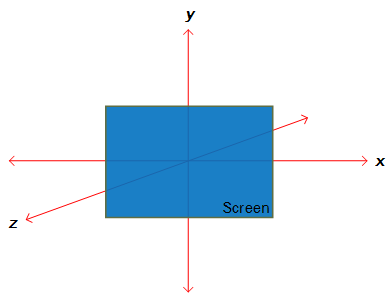
\includegraphics{images/implementation/threejs_coordinate_system}
	\caption[Three.js coordinate system]{Three.js coordinate system\protect\footnotemark.}
	\label{fig:threejs_coordinate_system}
\end{figure}

\footnotetext{\bibentry{microsoft2015threejs}}


	\subsection{Pan} {
	\label{sec:pan}

		This interaction is initiated when a \texttt{mousedown} event is fired on the canvas, followed by a \texttt{mousemove} event bound to the \texttt{window}. This simulates drag when pressing the left mouse button.

		As the user moves their pointer, the camera is translated in the x and y direction. This calculation relies on converting screen coordinates to world coordinates and normalising the value so it is a ratio of the viewport height, instead of both the width and height.

		Once the translation to the camera has been applied, the \texttt{origin} vector needs to be updated, which is used during rotation. An updated origin ensures there is no sudden movement when rotating, after panning the screen.

		Finally, when the user releases the left mouse button, a \texttt{mouseup} event is triggered which removes the event binding for \texttt{mousemove} on the \texttt{window}. 

	}

	\subsection{Rotate} {
	\label{sec:rotate}

		Rotation uses the same event chain as panning, except instead of listening to the left mouse click, it listens to the right.

		To rotate the camera, the cartesian coordinates need to be calculated from spherical coordinates, using the following formula in a right-handed mathetmatics system:

		%!TEX root = ../../report.tex

\begin{gather*}
	x = r\sin\phi\sin\theta \\
	y = r\cos\phi \\
	z = r\sin\phi\cos\theta
	\intertext{Where:}
	\begin{tabularx}{\textwidth}{@{}>{$}r<{$}@{\ :\ }X@{}}
		r & is the radial distance of the camera from the origin. \\
		\phi & is the polar angle, calculated by adding the delta phi angle with the angle from the y-axis. \\
		\theta & is the azimuthal angle, calculated by adding the delta theta angle with the angle from the z-axis around the y-axis. \\
	\end{tabularx}
\end{gather*}
	
	}

	\subsection{Zoom} {
	\label{sec:zoom}

		This navigation technique begins when a \texttt{wheel} event is triggered from the browser. A ratio of the delta value is taken and the camera is then translated by this amount.
	
	}

}

\section{Filtering} {
\label{sec:filtering_implementation}

	\todo{say how filtering was done, issues with extending it when I get around to implementing...should be a simple show/hide technique based on value}

}

\section{Configuration} {
\label{sec:configuration_implementation}

	Real-time configurations are best achieved by using shaders. Shaders are computer programs that perform shading on a graphics processing unit (GPU), making them highly efficient and well suited to parallel processing~\footnote{\bibentry{gerdelan2014shaders}}. Three.js provides abstracted materials that use shaders in the background, but this method does not easily facilitate highly customisable configurations or filter effects.

	The configurations were implemented with \href{http://workshop.chromeexperiments.com/}{dat.GUI}, a lightweight GUI for changing JavaScript variables in real-time. This tool is easy to use, setup and can modify shader uniforms automatically or by implementing \texttt{onChange} event handlers. dat.GUI can constrain input data and provides widgets for modifying values, colours and combo boxes. While this tool is great for modifying data on the fly, it has an outdated interface that does not always adapt well to particular colour schemes and designs. For this reason, the dat.GUI styles were modified to seamlessly integrate with the current system and the Material Design standards. The differences in design can be compared in Figure~\ref{fig:dat_gui} below.

	%!TEX root = ../../report.tex

\begin{figure}[H]
	\newcommand{\figurewidth}{0.4\textwidth}
	\newcommand{\figureheight}{7cm}
	\centering
	\begin{subfigure}[b]{\figurewidth}
        \figureborder{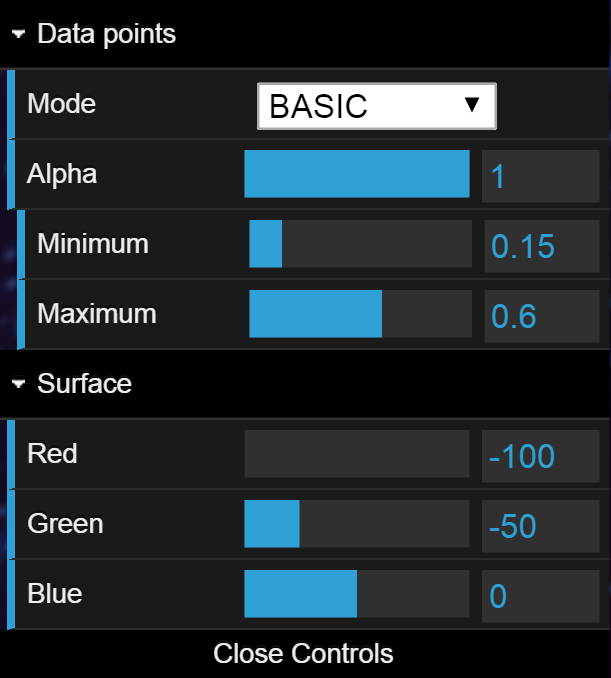
\includegraphics[width=\textwidth,height=\figureheight]{images/implementation/dat_gui/before}}
		\caption{Original dat.GUI interface.}
		\label{fig:dat_gui_before}
	\end{subfigure}
	\begin{subfigure}[b]{\figurewidth}
		\figureborder{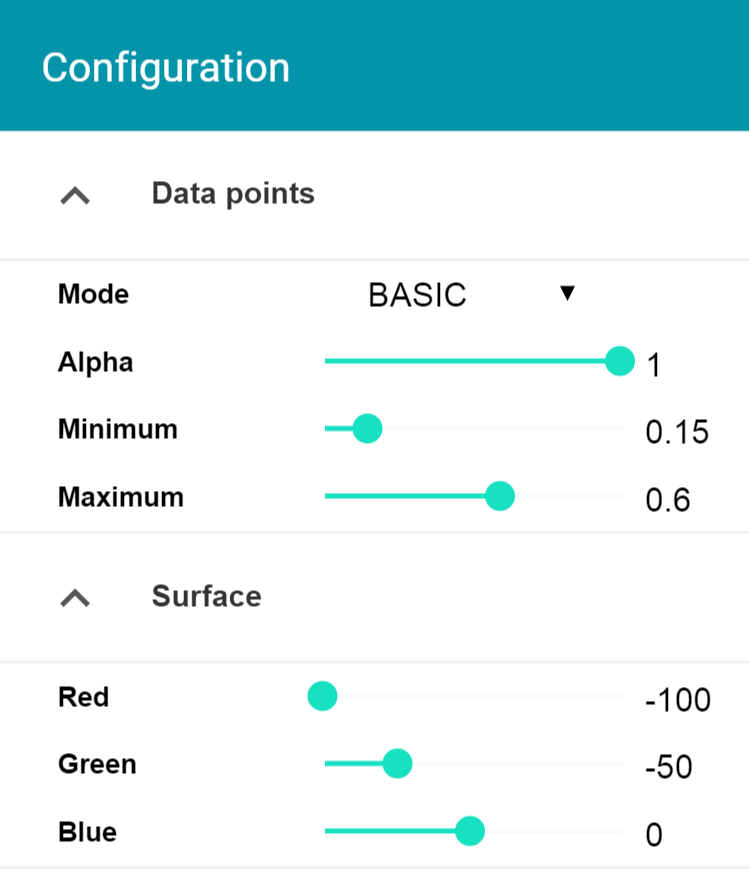
\includegraphics[width=\textwidth,height=\figureheight]{images/implementation/dat_gui/after}}
		\caption{dat.GUI interface after custom styling.}
		\label{fig:dat_gui_after}
	\end{subfigure}
	\caption[dat.GUI interface]{dat.GUI interface.}
	\label{fig:dat_gui}
\end{figure}


	The design for these configurations were continually refined during implementation. Initially, the dat.GUI sliders were to remain unchanged. However, these sliders added inconsistency to the interface in regards to colour scheme and filter design. Furthermore, the bold folder colours were eventually removed to reflect drawer layouts that conform to using light navigation colours, hover effects, and left floated icons.

}

\section{Data display} {
\label{sec:data_display}

	\todo{write about how the data displays were implemented - bunch of cubegeoms that get updated}

	% The development of these visualisations will involve using the established \href{http://threejs.org/docs/#Reference/Extras.Geometries/BoxGeometry}{BoxGeometry} and NURBS surface that are available in Three.js. The \href{http://threejs.org/examples/webgl_geometry_nurbs.html}{NURBS example}, as displayed in Appendix~\ref{app:nurbs}, proves that it is possible to render a smooth 3D surface. This can be applied to represent a heat map and if there lie difficulties in implementing this, then a simpler representation can be modelled.

}

\section{Information display} {
\label{sec:information_display}

	\todo{say how this was implemented - raycaster in requestanimframe, toggles one element to hide/show so nothing new in dom is added (more performant)}

	%!TEX root = ../../report.tex

\begin{figure}[H]
	\centering
	\newcommand{\figurewidth}{0.4\textwidth}
	\centering
	\begin{subfigure}[b]{\figurewidth}
        \figureborder{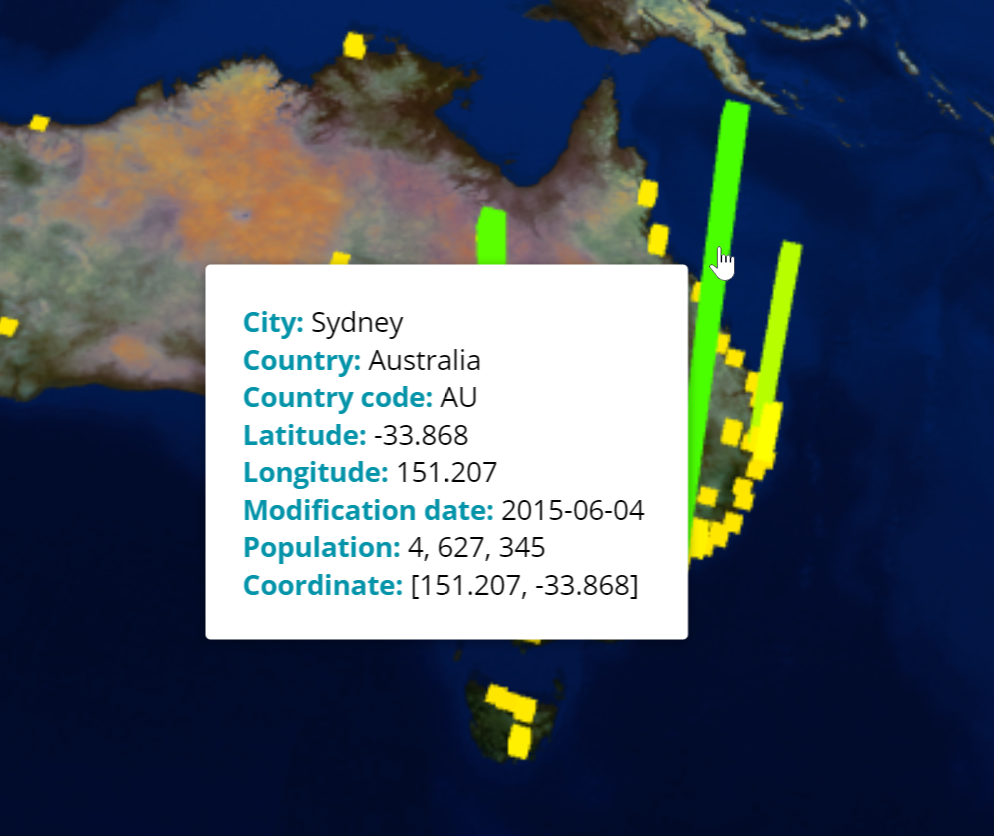
\includegraphics[width=\textwidth]{images/implementation/information_display/population}}
		\caption{Information display for population data.}
		\label{fig:information_display_population}
	\end{subfigure}
	\begin{subfigure}[b]{\figurewidth}
		\figureborder{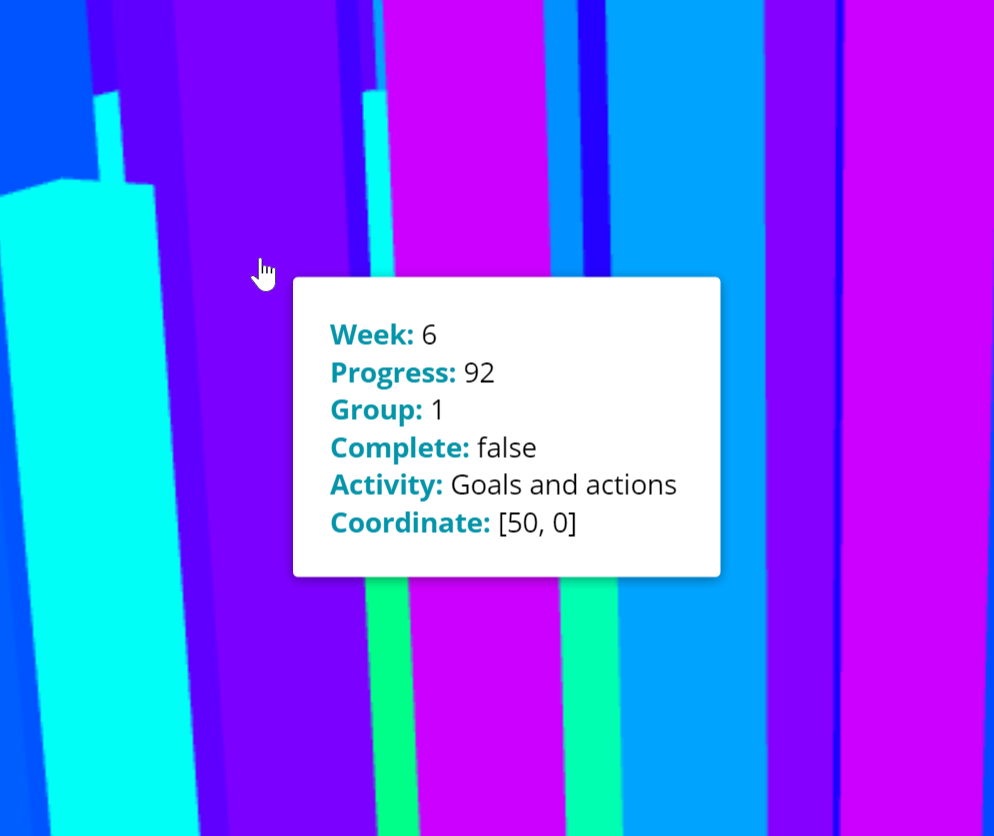
\includegraphics[width=\textwidth]{images/implementation/information_display/student}}
		\caption{Information display for student data.}
		\label{fig:information_display_student}
	\end{subfigure}
	\caption[Information display]{Information display hover effect.}
	\label{fig:information_display}
\end{figure}


}

\section{Flat surface} {
\label{sec:flat_surface}
	
}

\section{Round surface} {
\label{sec:round_surface}
	
}

\section{Grid} {
\label{sec:grid}
	
}

\todo{Map to project outcomes??}